A programmable computer is a gadget without precedent.
It can be appreciated from many perspectives.
For example, it can be viewed as an engineering marvel of ever-increasing capacity;
as a medium for new flashy applications;
or as the machine-independent scientific discipline that forms its foundations~\cite{dijkstra1979a,hoare2006}.
This dissertation focuses on the intellectual challenge of {programming} these gadgets.

\begin{quotation}
\noindent This challenge seems unique in the combination of the possibility for
unmastered complexity -- programs are among the most complex things ever
conceived -- and the ultimate, but misleading, simplicity of a world of zeros
and ones alone~\cite{dijkstra1979a}.
\end{quotation}

Programming languages provide us an interface for crafting programs.
The languages are a useful \emph{abstraction layer}, because they relieve us from working directly with 0s and 1s.
A program is written in {high-level} language that is (intended to be) intelligible to humans.
The program is then \enquote{translated} (compiled), from the high-level language to 0s and 1s, for processing by computers.
However, the abstraction provided by programming languages does nothing to reduce the intellectual challenge involved in programming~\cite{dijkstra1979b}.
If we write a (syntactically legal) faulty program, we are at the mercy of our faulty creation.

\paragraph{Equivalence.}
One fascinating feature about programs is that we can write multiple distinct programs that compute the same result.
Two programs $\sem{p_1}$\symbo{funprog} and $\sem{p_2}$\symbo{funprog} are functionally \emph{equivalent}\index{functional equivalence}, \ie \(\sem{p_1} \equiv \sem{p_2}\)\symbo{equiv}, iff for every possible input \(i\), \(\sem{p_1}(i) = \sem{p_2}(i)\)\symbo{funprog}.
When we want functional equivalence, we must fix the program input and output, but can alter \emph{how} the result is computed.
A scientifically inclined reader will recognize functional equivalence as multiple algorithms computing the same function.
A software engineer will recognize it in the art of \ndx{refactoring}.

To demonstrate the idea, consider the two programs in~\autoref{lst:intro}.
The variable \pr|bit| is either \(0\) or \(1\).
By visual inspection, it is obvious that the programs look different.
Yet, for all values of variables \pr|X| and \pr|Y|, they compute the same result.%
\footnote{This is an informal claim. It will be revisited in~\autoref{subsubsec:sm-tool-examples}.}
The result is stored in variable \pr|Z|.
Thus, the programs are functionally equivalent.

\begin{center}
\captionsetup{type=lstlisting}
%! suppress = FileNotFound
\begin{minipage}{.3\textwidth}
\lstinputlisting[nolol,label={lst:p1},frame=none,numbers=none,aboveskip=0pt,belowskip=0pt]{equiv1.imp}
\end{minipage}%
\hspace{5em}%
%! suppress = FileNotFound
\begin{minipage}{.4\textwidth}
\captionsetup{type=lstlisting}
\lstinputlisting[nolol,label={lst:p2},frame=none,numbers=none,aboveskip=0pt,belowskip=0pt]{equiv2.imp}
\end{minipage}
\captionof{lstlisting}[Equivalent programs]{Equivalent programs.}
\label{lst:intro}
\end{center}

It is natural to ask, \enquote{which program is better?}
The left is free of arithmetic and, for a human, reads more intuitively and is easier to understand.
Such clarity is a useful criterion if the program is intended for frequent visual inspection.
However, we may not care about readability.
Many programs, like the ones generated by a compiler, are never read by humans.
The program on right has the advantage that it eliminates the conditional branch and always evaluates the full arithmetic expression.
Such features are desirable for software security.
Therefore, choosing the preferable program form depends on semantics.
What exactly do we mean by \enquote{better} and how do we quantify measure such metrics?

\paragraph{Non-functional properties.}
The quality attributes of programs, \ie features that extend beyond functional behavior, are called \emph{\ndx{non-functional properties}}.
Non-functional properties include attributes like program security and resource consumption.
Throughout the dissertation, a major topic of interest is inspecting programs as mathematical objects \wrt non-functional properties.
Among the direct goals are developing techniques that enable quantifying the properties.
Furthermore, instead of trusting informal claims, like the one of equivalence, we want rigorous confirmation that the stated properties truly hold in the inspected program(s).

\vspace{1em}\noindent{}Thus the challenge of programming involves more than the art of \emph{writing} programs. Reasoning about the program \emph{behaviors} is an independent scientific challenge.

\subsection{Dissertation core topics}
\label{subsec:dissertation-themes}

Embracing the natural ambiguity in programs brings us to the topics of static program analysis and formal methods.
These two are foundational themes of this dissertation.
For an enhanced sense of adventure, and to make the dissertation exploration worthy of a multi-year doctoral study, we add to the mix \emph{implicit computational complexity}.

\paragraph{Static program analysis and formal methods.}
Program analysis provides the techniques to inspect programs and check whether they satisfy some desirable behavioral criterion.
The focus in this dissertation is to analyze programs statically, \ie by how the programs are written syntactically.
In static program analysis we make judgements about how the program will behave when it is executed, but without executing the program.
Formal methods complements program analysis by providing the mathematical techniques needed to obtain rigorous guarantees.
With formal methods it is possible to provide \emph{proofs} about the conclusions of program analysis.
This way, we can swap informal claims to maximally strong assertions.

\paragraph*{Implicit computational complexity.}
The core idea of implicit computational complexity (ICC) is to quantify computational power through programming languages.
Although ICC can be viewed from many perspectives, in the scope of this dissertation, its role is to provide a conceptual \enquote{toolbox} for constructing techniques of static program analysis.
Very broadly, ICC finds ways to characterize program properties---mainly resource consumption---by introducing a restriction at the level of a programming language.
The restriction is such that it gurantees the target property holds in every expressible program.
Thus, programming languages become a \emph{mechanism} to guarantee ideal runtime behavior.
There are multiple compelling motivations for this approach.
For example, ICC drives better understanding of resource consumption and provides natural ways to express and control resources usage of programs~\cite{kristiansen2017}.
Because behavioral guarantees are part of the language design, this creates a temporal shift that enables reasoning about properties \emph{before} any program exists.
In principle, this removes the need for post-analysis of programs.
However, materializing these ideas requires deeper investigations of implicit computational complexity.

\begin{mdframed}[backgroundcolor=conceptbase,linecolor=concept,nobreak=true]
The dissertations is about \textbf{static program analysis}, ideally with
\textbf{formal guarantees}, and starting with \textbf{implicit computational
complexity} -- a family of programming language-based techniques that can
provide behavioral guarantees by construction.
\end{mdframed}

\subsection{Addressed Problem}
\label{subsec:problem}

Given the many compelling ideological perspectives, there exists a long series of theoretical results in implicit computational complexity, reviewed in~\autoref{icc-theories}.
These works focus primarily on \emph{defining} theoretical systems.
There are substantially fewer explorations of \emph{applications} of those theories -- see Sections~\ref{resource-analysis-tools} and~\ref{icc-sec} for related presentations.%
\footnote{An \emph{application} refers to any use case beyond complexity theory, including implementation.}
The difference in the allocated efforts could be explained by many factors, including the following challenges.%
\footnote{These are opinions and arise from observations and conversations about the process of doing research; it is doubtful they are annotated in literature.}

\begin{enumerate}

\item Broad insight is required to identify suitable application domains -- as
      evidenced by, \eg \ndx{Parikh's Theorem} in \ndx{automata theory}.%
      \footnote{The classic Parikh's Theorem is about letter-counting and language expressiveness.
      Its usefulness in applications was enabled only \emph{decades later} by the development of efficient algorithms.
      Since then,  it has been exploited in a range of applications like SMT solvers, verification of cryptographic protocols and concurrent programs, and query evaluations in graph databases~\cite[pg. 2]{hague2024}.}

\item Applying any pure theory reveals the shortcomings of the theory.
      It is extremely difficult to design a useful theory without considering its implementation.

\item An application may alter the research domain; \eg from theoretical computer science to verification, program analysis, formal methods, \etc
      In other words, it requires communicating findings to (new) audiences, who may be motivated differently to assess the usefulness of the findings.

\end{enumerate}

Certain application motivations are specific to ICC\@.
Restricting a programming language sacrifices \ndx{Turing-completeness}.
A non-Turing-complete programming language makes certain programs inexpressible.
The task of writing (or finding) a satisfactory program is then delegated to the software engineer~\cite[p. 14]{moyen2017}.
If the ICC restriction is too strong, it is difficult, or perhaps impossible, to express natural algorithms.
This leads to a tradeoff between theoretical soundness, \ie providing a guarantee, and expressiveness~\cite{feree2018}.
It is justifiable to ask, \emph{what can we do with such restricted programming languages?}.%
\footnote{See \url{https://stackoverflow.com/questions/315340} for an inspirational warm-up.}

Through applications, we can stress test and pinpoint the limitations and capabilities of ICC systems, and discover new use cases in other domains.
The guiding hypothesis of the dissertation research is summarized in~\autoref{fig:hypothesis}). Every manuscript in this dissertation is an instantiation of this hypothesis.

\begin{figure}[h]
\begin{mdframed}
\paragraph*{Main hypothesis.}
Implicit computational complexity offers applied utilities when lifted from the
theoretical domain.
\end{mdframed}
\caption[Main hypothesis summarized]{Main hypothesis.}
\label{fig:hypothesis}
\end{figure}

\subsection{Dissertation Goals}\label{subsec:specific-aims}

In support of the main hypothesis, there are four research goals (G\#).

\begin{enumerate}[label={\textbf{G\arabic*.}}]

\item\emph{Extend applied capabilities of ICC in automatic program analysis and verification.}
The motivation is to show that ICC theories can provide new practical (orthogonal) techniques of automatic program analysis and help guarantee programs satisfy desirable properties.

\item\emph{Take ICC a few steps closer to integration into real-world software development workflows.}
The integration would drive theoretical improvement, enhance relevance of ICC techniques, and motivate thinking about ICC from fresh perspectives.

\item \emph{Initiate conversations on the relevance of ICC applications.}
Improvements in ICC are typically achieved by showing improvement in expressiveness.
The common strategy---used \eg in~\cite[p.16--17]{hainry2023},~\cite[p. 17]{jones2009}, and~\cite[p. 147]{feree2018}---is to show that the newly presented system gives a guarantee for some subset of programs that were not expressible previously.
However, this strategy is limited in quantifying practical usefulness of the ICC systems.
Particularly, it does not account for the \enquote{methodological cost} at which the improvement is achieved.
Applications would provide complementary insight and metrics to assess the capabilities of ICC systems.

\item \emph{Expose ICC to broader research communities.}
The expectation is that wider propagation of ideas leads to discovery of new use cases.
Moreover, through wider familiarity, is eases communication about ICC results.

\end{enumerate}

\subsection{Manuscripts and Research Questions}
\label{subsec:conn-papers}

To make the abstract dissertation hypothesis and research goals more concrete, we define two research directions.
Broadly, one focuses on automatic resource analysis, and the other investigates uses of ICC to ensure other program properties, beyond complexity.
These directions are visualized in~\autoref{fig:conn_papers}. An alternative way to think about these directions is that
\begin{enumerate*}
\item we apply the systems in the originally designed ways (on left), and
\item we aims to discover unexpected applications (on right).
\end{enumerate*}

\begin{figure}[p]
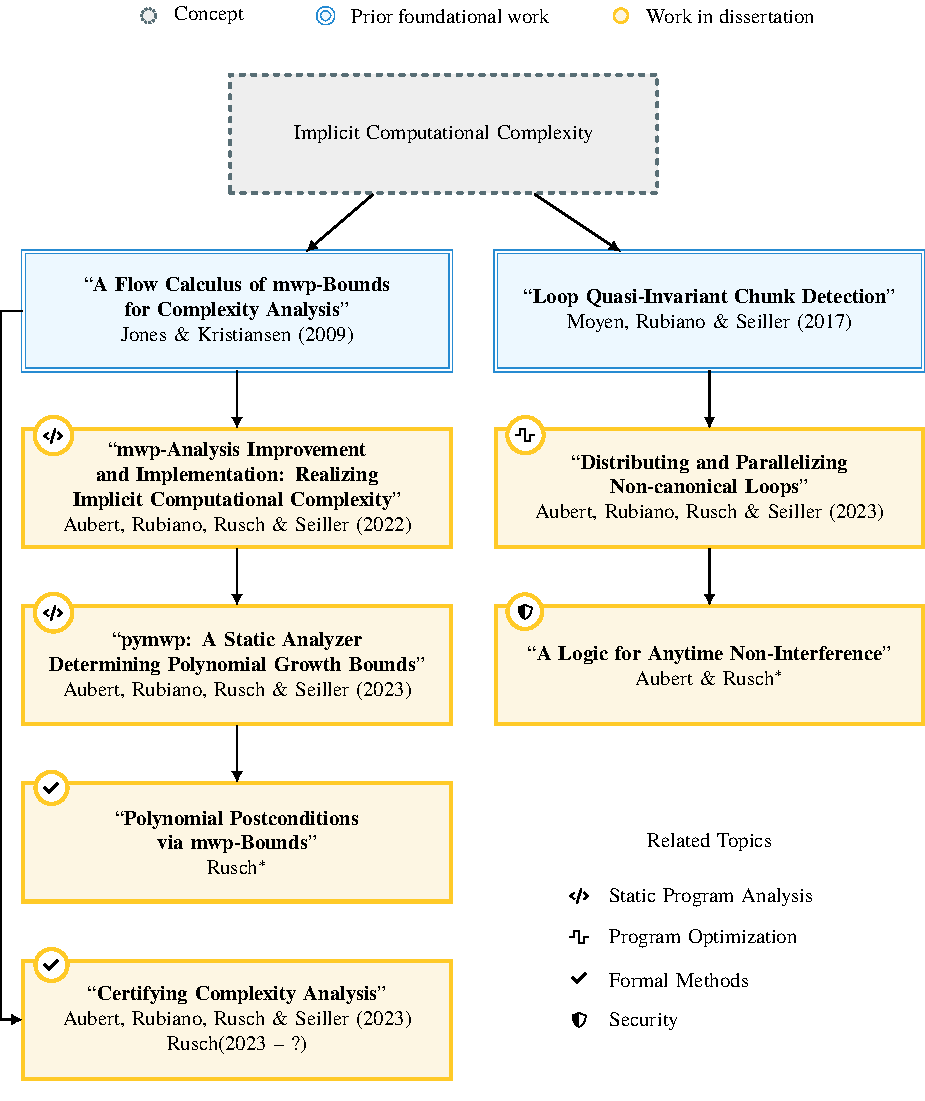
\includegraphics[width=\linewidth,keepaspectratio]{fig_conn_papers}\vspace{1em}
\caption[Dissertation manuscripts and their associations]
{Dissertation manuscripts and their associations.}
\label{fig:conn_papers}
\end{figure}

\paragraph*{Automatic resource analysis.}
\index{mwp-calculus}

In the first direction, we focus on the flow calculus of mwp-bounds of~\textcite{jones2009}.
It is a canonical example of an ICC system for analysing variable value growth (data size) in \ndx{imperative programs}.
The flow calculus is introduced in detail in~\autoref{flow-calculus}.

Relating to the flow calculus, we define three research questions.
\begin{description}
\item[RQ1] Can we develop an \emph{automatic} program analysis based on the flow calculus?
\item[RQ2] Given its paper proofs, is the theory correct, \ie can we prove formally the soundness of the flow calculus?\index{soundness of mwp-calculus}
\item[RQ3] Assuming the theory can be automated, what are its use cases?
\end{description}

The manuscripts demonstrate the utility of the calculus, first in static program analysis and then extending to formal methods.%
\footnote{Due to Augusta University policies, one manuscript is in the appendix.
The placement should not distract from the significance of the work, as several other manuscripts follow from it.}
The manuscripts supports all dissertation goals.
The implementation of the calculus, RQ1, supports G1--G3.
A proof of its soundness (RQ2), and its extension to formal methods that follows from RQ3, support G4.

\paragraph*{Analyzing extended program properties.}

The second direction is inspired by \enquote{Loop Quasi-Invariant Chunk Detection}~\cite{moyen20172}.
In the original formulation, the idea is to identify fragments (blocks) of loops, whose variables become invariant after a finite number of iterations.
Such loop \ndx{quasi-invariant} code blocks can then be lifted from the loop.
The program transformation improves the loop's complexity profile if the lifted block is a nested loop.
For convenience, we refer this technique as the \emph{QI framework}, after the quasi-invariants.

This original QI framework is not presented in this dissertation.
This is because each refinement changes the behavior of the system.
It is therefore necessary to fully re-define the system each time.
The manuscripts in Sections~\ref{sec:vmcai} and~\ref{sec:anytime} provide the technical details.

Using the QI framework, we define two research questions.
\begin{description}
\item[RQ4] How to develop a program transformation to increase parallelization potential?
\item[RQ5] How to use it to analyze security properties, specifically non-interference?
\end{description}

The research questions change the orientation from complexity theory to other application domains.
Critically, the original complexity result may be lost, but some other guarantee is gained instead.
On the surface, the research questions appear to be about properties, but more deeply they are about understanding the underlying theory and its flexibility.

Both goals are practically motivated. The expected deliverables support G1 and G2. Moreover, they are strongly oriented to support G4.

\paragraph*{Related topics.}
Each manuscript connects implicit computational complexity with a related research topic.
The topics include static program analysis, security, program optimization, and formal methods.
Each dissertation manuscript is decorated with an icon that denotes the related topic.

\paragraph*{On manuscript authorship.}
The manuscript authors are listed in alphabetical order.
The manuscripts in Chapters~\ref{published-manuscripts}--\ref{ch:unpublished-research} are \enquote{first author} works.
The manuscripts in~\autoref{app:additional-manuscripts} are \enquote{non-first author} works.
The contributions of the co-authors are detailed in~\autoref{app:sec:coauth}.

\paragraph*{On manuscript peer review.}
The entire Chapters~\ref{published-manuscripts},~\ref{ch:unpublished-research},~\ref{ch:summary}, and~\ref{app:additional-manuscripts} have been peer-reviewed.
In other words, the only new content sections are Chapters 1 and 4, Introduction and Discussion.

\begin{itemize}

\item The published works, in Chapters~\ref{published-manuscripts} and~\ref{app:additional-manuscripts}, were inspected by 7--10 reviewers before acceptance.

\item The unpublished works, in \autoref{ch:unpublished-research}, have been reviewed by 3--6 reviewers thus far.
Preliminary versions of most unpublished works have been accepted and presented at respectable workshops.
However, the unpublished research must be viewed with some caution.
They all have some limitation that prevents their inclusion in the chapter of published manuscripts.

\item \autoref{ch:summary} is a standalone extended abstract about the full-length dissertation.
It has been peer-reviewed and presented at \href{https://2025.ecoop.org/track/ecoop-2025-doctoral-symposium}{the doctoral symposium} of \href{https://2025.ecoop.org}{the European Conference on Object-Oriented Programming (ECOOP)} 2025.

\end{itemize}

\subsection{Important Tips for Interacting With This Dissertation}
\label{subsec:tips}

This dissertation contains three, varying-length versions of its contents.

\begin{mdframed}[backgroundcolor=paperbase,linecolor=paper,nobreak=true]
\begin{enumerate}[wide, labelwidth=!, labelindent=0pt]
\item The \textbf{\hyperref[abs]{abstract}} contains the highlights only.
\item \textbf{Chapters~\ref{introduction}--\ref{ch:discussion} and~\ref{app:additional-manuscripts}} form the full-length presentation.
\item \textbf{\autoref{ch:summary}} is a standalone, extended summary of the full presentation.
\end{enumerate}
\end{mdframed}

Choose the version that best matches your needs.

\subsubsection{Software Artifacts and Data Availability}

Each published manuscript included in the dissertation has an associated software artifact.
Similarly, the dissertation has a companion artifact that allows, \eg executing included code fragments.
How to locate the artifacts is explained in~\autoref{app:sec:artifacts}.
Therefore, each manuscript consists of more than just the text pages of the dissertation.

All software developed as part of this dissertation is publicly available.
The software is archived, according to the policies of the Association for Computing Machinery~\cite{acm_badging}, for long-term retention.
The software is achieved even if the publication venue did not provide an artifact evaluation round.

\subsubsection{Notational Conventions}

\paragraph*{Syntax and code blocks.}
Inlined syntactic constructs (variables, expressions, commands, \etc) are typeset in \pr|teletype|.
Larger code blocks are displayed in dedicated listings.
The listings will display, in bottom right corner, the associated programming language, or context, according to~\autoref{tab:pls}.
In the table, \emph{version} is the release version assumed in the dissertation listings.
Pseudo-languages have no version.
Plain text listings describe command outputs.
They are labelled \enquote{output}.
The \ndx{Rocq} Prover is undergoing a name change from the former name Coq\index{Coq|seealso{Rocq}}.
We will use the new name whenever possible.

\begin{table}[h]
\begin{center}
\begin{tabular}{@{}lllc@{}}
\toprule
\multicolumn{2}{@{}l}
{\textbf{Language}} &
\textbf{Description} &
\textbf{Version} \\
\midrule
\langclr{cc}        & C           & the \ndx{C} programming language & C99 \\
\langclr{ccstar}    & C*          & imperative C-like pseudo-language & -- \\
\langclr{cces}      & CES         & \ndx{cost equation system} &  -- \\
\langclr{ccmd}      & cmd         & executable shell (terminal) command & --  \\
\langclr{cdafny}    & Dafny       & the \ndx{Dafny} programming language & 4.10.0 \\
\langclr{cimp}      & Imp         & imperative language of \ndx{mwp-calculus} & -- \\
\langclr{cjava}     & Java        & the \ndx{Java} programming language & SE 24 \\
\langclr{compcode}  & OMP         & C code that includes \ndx{OpenMP} directives & 6.0 \\
\langclr{crocq}     & Rocq        & the \ndx{Rocq} interactive theorem prover & 8.20.1 \\
\langclr{cmathc}    & SSReflect   & the \ndx{SSReflect} proof language & 2.4.0 \\
\langclr{cwhile}    & While       & simple imperative while language & -- \\
\bottomrule
\end{tabular}\end{center}
\caption[The programming languages of code listings]
{The programming languages used in code listings.}
\label{tab:pls}
\end{table}

\paragraph*{Line numbers.}
References to specific line of source code, or an algorithm, begin with L, for \underline{l}ine.
The L is followed by a number, or a numeric range, that specifies the rows of interest.
For example, L3 means \enquote{line number 3} and L10--12 means \enquote{lines 10 through 12}.

\paragraph*{Distinguishing variable states.}
We will often want to refer to the same variable in different states of computation.
In the style of \ndx{Z specification language}~\cite{spivey1992}, we use notation that identifies the \emph{new (post) states}.
A plain variable refers to a state where the variable holds its {initial} value.
A variable with a postfix decoration \pr|'| refers to a state where the variable holds its {final} value.
For example, \pr|X| refers to the initial value and \pr|X'| refers to the final value.

\subsubsection{Term and Notational Indices}

The dissertation includes three indices.
The Term Index (\autoref{sec:app:index}) lists technical terms and their most prevalent uses.
The other two indices are for acronyms and symbolic notations.
Acronyms are generally defined at first use.
After that, the long form can be located in the Index of Acronyms (\autoref{glo:acr}).
A similar reference is available for symbolic notations in the Symbol Index (\autoref{glo:symb}).

\subsubsection{Dynamic Bibliographic Entries}

Some bibliography entries refer to resources that are not traditional scientific papers, like software, web pages, lecture notes, \etc.
To improve the long-term availability of such dynamic bibliographic entries, they are pre-emptively deposited in online archives.

\paragraph*{Written documents.}
Web pages and PDF files are archived at the \ndx{Internet Archive}'s \ndx{Wayback Machine}.
To recover a document from the Internet Archive, substitute \pr|<URL>| by the document's URL\@.
\begin{center}\pr|https://web.archive.org/web/<URL>|\end{center}
A few cited documents could not be archived in the Internet Archive.
Those documents are archived with the dissertation companion artifact (\autoref{tab:pub-artifacts}).

\paragraph*{Software repositories.}
Version-controlled third party software repositories are archived at \href{https://softwareheritage.org}{\ndx{Software Heritage}}.
For a repository hosted at \pr|<URL>|, the recovery address is:%
\begin{center}\pr|https://archive.softwareheritage.org/browse/origin/directory/|\mbox{\pr|?origin_url=<URL>|}\end{center}

\paragraph*{Example: recovering archived documents.}\mbox{}

The following \href{https://types22.inria.fr/files/2022/06/TYPES_2022_paper_14.pdf}{URL} is fragile and may disappear in the future.
\begin{center}
\begin{minipage}{\textwidth}
%! suppress = EscapeUnderscore
\begin{cmdlisting}*[nolol]
https://types22.inria.fr/files/2022/06/TYPES_2022_paper_14.pdf
\end{cmdlisting}
\end{minipage}
\end{center}

If a request of the original document fails, the following \href{https://web.archive.org/web/https://types22.inria.fr/files/2022/06/TYPES_2022_paper_14.pdf}{Internet Archive address} produces the same document.
\begin{center}
\begin{minipage}{\textwidth}
%! suppress = EscapeUnderscore
\begin{cmdlisting}*[nolol]
https://web.archive.org/web/https://types22.inria.fr/files/2022/06/TYPES_2022_paper_14.pdf
\end{cmdlisting}
\end{minipage}
\end{center}